\documentclass{article}
\usepackage{graphicx} % Required for inserting images
\usepackage{sidecap}
\usepackage{wrapfig,lipsum}
\usepackage[utf8]{inputenc} %lettere accentate da tastiera 
\usepackage[T1]{fontenc} % higher quality font encoding

%load the font and set it to default
\usepackage{amsmath,amsthm,amsfonts,amssymb}
\usepackage[english,italian]{babel}
\usepackage{amsmath}
\usepackage{url}
\usepackage{geometry}
\geometry{a4paper,top=3cm,bottom=3cm,left=3.5cm,right=3.5cm,%
	heightrounded,bindingoffset=5mm}
\usepackage{tikz}
\usepackage[x11names]{xcolor}
\usepackage{tcolorbox}
\tcbuselibrary{theorems}

\usepackage{hyperref}
\hypersetup{
	colorlinks=false,
	linkcolor=blue,
	filecolor=magenta,      
	urlcolor=blue,
	pdftitle={Analisi II},
	pdfpagemode=FullScreen,
}
\usepackage{enumitem}

\newtheorem{teorema}{Teorema}[subsection]

\theoremstyle{definition}
\newtheorem*{definizione}{Definizione}

\newtheorem*{proprieta}{Proprietà}
\newtheorem*{corollario}{Corollario}
\newtheorem*{formula}{Formula}
\newtheorem*{proposizione}{Proposizione}
\newtheorem{prop}{Proposizione}
\newtheorem*{lemma}{Lemma}

\newtheorem{nulla}{}
\newtcbtheorem[number within=section]{teo}{Teorema}{colback=black!5 ,colframe=black!90 }{}
\newtcbtheorem[number within=section]{teo1}{}{colback=black!5 ,colframe=Burlywood4!80 }{}
\newcommand{\R}{\mathbb{R}}
\newcommand{\D}{\mathbb{D}}
\newcommand{\V}{\mathbb{V}}
\newcommand{\K}{\mathbb{K}}
\newcommand{\w}{\mathbb{W}}
\newcommand{\C}{\mathbb{C}}
\newcommand{\norma}{||\cdot||}\usepackage{mathtools}
\newcommand{\Rn}{\R^n}
\newcommand{\la}{\lambda}
\newcommand{\on}{^{\perp}}
\newcommand{\A}{\mathbb{A}}
\newcommand{\xb}{\overline{x}}
\newcommand{\fn}{f: A\subseteq \Rn \rightarrow \R}
\newcommand{\fnn}{f: A\subseteq \Rn \rightarrow \Rn}
\newcommand{\fnm}{f: A\subseteq \Rn \rightarrow \R^m}
\newcommand{\s}{$\Sigma$}
\renewcommand{\labelitemi}{$\star$}
\title{Analisi II }
\author{Luca Mombelli}
\date{2024-25}

\begin{document}
	
	\maketitle
	\tableofcontents
	\newpage
	
	\section{Topologia}
	\begin{definizione}
		\textit{Palla (aperta)} \\ 
		Sia $x\in \Rn \ e \ r > 0$ chiamiamo palla aperta di centro x e raggio e l'insieme : 
		$$B(x,r)=\{y\in \Rn \ | \  ||y-x||<R\}$$
	\end{definizione}
	\begin{definizione}
		\textit{ Aperto/chiuso} 
		\begin{itemize}
			\item Sia $A \subseteq \Rn$ diciamo che A è aperto se 
			$$\forall x \in A \ \exists r> 0 \ t.c \ B(x,r)\subseteq A $$
			\item Sia $C \subseteq \Rn$. Diciamo che C è chiuso se $\Rn \setminus C$ è aperto
		\end{itemize}
	\end{definizione}
	Esistono insieme che non sono ne aperti ne chiusi , ad esempio : \\$A=\{(x_1,x_2)\in \R^2 \ | \ 0<x_1<1 \ \ 0\leq x_2 \leq 1 \} $ 
	\begin{figure}[h]
		\centering
		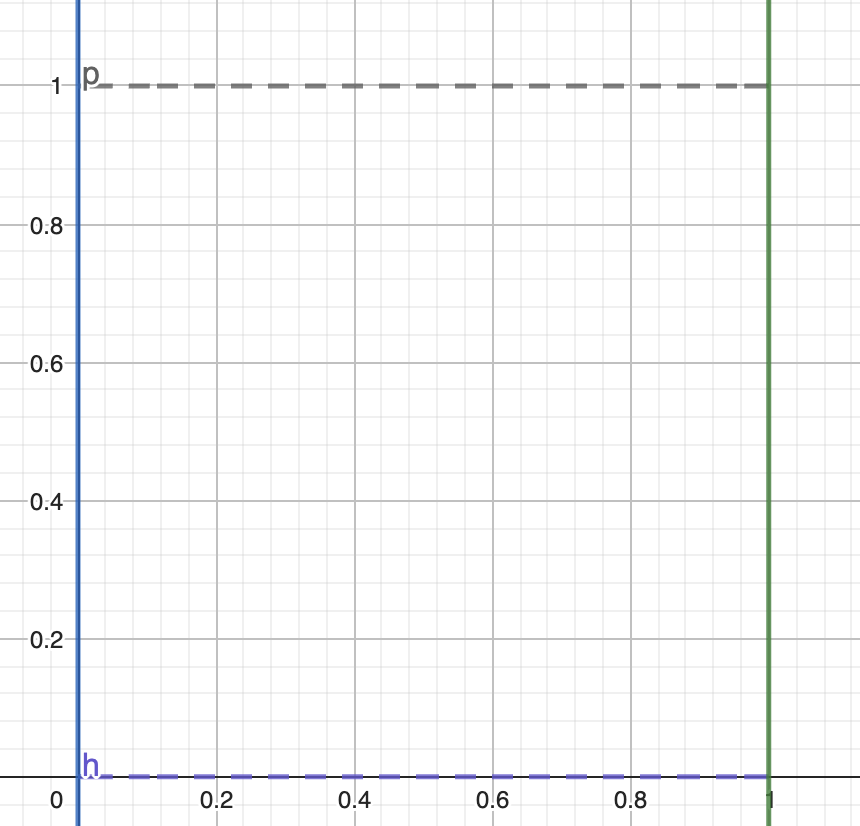
\includegraphics[scale=0.25]{immagini/Screenshot 2024-10-02 alle 19.54.09.png}
		\caption{esempio}
		\label{fig:es}
	\end{figure} \\
	Inoltre vi sono unicamente due insieme che sono sia aperti sia chiusi : $\emptyset\ \ \ \  \Rn$\\
	Osservazione : A è aperto se $A=A^0$\\
	A è chiuso se $A=\overline{A}$ \\
	se A è aperto , allora E non contiene $\partial A$\\
	se A è chiuso , allora A contiene $\partial A$ \\
	$A^0 \cup \partial A = \overline{A}$
	
	\begin{definizione}
		\textit{Intorno} \\
		Sia $ x \in \Rn$ diciamo intorno di x un qualsiasi insieme aperto $U\subseteq \Rn$ che contiene x. \\In particolare B(x,r),r>0 , è detto intorno \textbf{sferico} di x. 
	\end{definizione}
	\begin{definizione}
		Punto di accumulazione \\
		$x \in \Rn$ è un punto di accumulazione di $E \subseteq \Rn$ se in ogni intorno sferico centrato in x $B(x,r)$ esiste almeno un punto di E diverso da x
	\end{definizione}
	\begin{definizione}
		Sia $E \subseteq \Rn$ 
		\begin{itemize}
			\item$x \in \Rn$ è un punto interno per E se $\exists r>0$ t.c $B(x,r) \subseteq E$ definiamo l'interno E come $E^0=${punti interni di E}
			\item $x \in \Rn$ è un punto di frontiera per E se $\forall r>0$ t.c 
			\begin{gather*}
				B(x.r)\cap E \neq \emptyset \\
				B(x,r) \cap ( \Rn \setminus E ) \neq \emptyset 
			\end{gather*}
			definiamo la frontiera di E come  $\partial E$={punti di frontiera di E}
			\item $ x \in \Rn$ un punto esterno per E se $\exists r > 0$ t.c $B(x,r) \subseteq \Rn \setminus E$
			\item Definiamo chiusura di E l'insieme $\overline{E}= E \cup \partial E $
		\end{itemize}
	\end{definizione}
	Esempio : $E=[1,2) \ \ \ \ \partial E = \{1,2\} \ \ \ E^0=(1,2) \ \ \ \ \ \overline{E}=[1,2]$
	\begin{proposizione}
		Sia $\{A_n\}_n$ una famiglia di insiemi aperti. Allora : 
		$$\bigcup_{n=1} ^{\infty} A_n \ \text{è} \ aperto , \hspace{0.2cm} \bigcap_{n=1}^N A_n\ \text{è}\ aperto \ N > 0 $$
		
		
		Sia $\{A_n\}_n$ una famiglia di insiemi chiusi. Allora : $$\bigcup_{n=1} ^{N} A_n \ \text{è} \ chiuso , \ \bigcap_{n=1}^{\infty} A_n\ \text{è} \ chiuso \ N > 0 $$
	\end{proposizione}
	
	\begin{proposizione}
		Sia $C \subseteq \Rn$- Allora C è chiuso $\leftrightarrow \forall \{x_k\}_k \subseteq C \ ,\ x_k \rightarrow \overline{x} , \ allora \ \overline{x} \in C $ \\
		C contiene i limiti delle sue successioni convergenti 
	\end{proposizione}
	\begin{definizione}
		\textit{Insieme limitato \\
		}  Sia $ E \subseteq \Rn$. Diciamo che E è limitato se $\exists R > 0 $ t.c $E \subseteq B(0,R)$\\ ($\exists R > 0 \ t.c \ ||y|| < R \ \ \forall y \in E)$
	\end{definizione}
	\begin{definizione}
		\textit{    Insieme finito \\
		}    Sia $E\subseteq \Rn$ è finito se la cardinalità di E è minore di +$\infty$
	\end{definizione}
	\begin{definizione}
		Insieme convesso \\ \label{def:1}
		Sia $A \subseteq \Rn$. Diciamo che A è convesso se per ogni coppia di punti $x,y \in A$ , il segmento che connette x e y sta interamente in A.
	\end{definizione}
	\begin{definizione}
		Insieme connessi per archi \\ \label{def:2}
		Sia $E \subseteq \Rn$ , diciamo che E è connesso per  archi se $\forall x,y \in E $ esiste un arco di curva continua interamente contenuto in E con estremi x e y 
	\end{definizione}
	\begin{definizione}
		Insieme semplicemente connesso\\
		Sia $\Omega \subseteq \R^n$ , $\Omega$ è semplicemente connesso se è connesso (per archi) e ogni curva chiusa interamente contenuta in $\Omega$ può essere ridotta a un punto mediante deformazioni continue senza uscire da $\Omega$
	\end{definizione}
	\section{Limiti}
	
	\begin{definizione}
		\textit{Limite per successioni}\\
		Sia $\{x_k\}_k \subset \Rn $ e sia $x\in \Rn$ . Diciamo che 
		$$x_k\rightarrow \overline{x} \ per \ k \rightarrow +\infty \ oppure \lim_{k\rightarrow +\infty}x_k=\overline{x}$$
		\begin{align*}
			\ \forall \epsilon > 0 \ \exists N > 0 \ \ t.c. \ \ & x_k \in \ B (\overline{x},\epsilon) \ \  \forall k > N \\
			&||x-\overline{x}|| < \epsilon
		\end{align*}
		$x_k \rightarrow \overline{x} \rightarrow$ ogni elemento del vettore converge
	\end{definizione}
	\begin{definizione}
		Continuità \\
		$f:\ E\subseteq \Rn \rightarrow \R^m $ e sia $ \overline{x}\in E$ è continua in $\overline{x}$ se 
		$$\forall \{x_k\}_k \subseteq E , x_k \rightarrow \overline{x} \ allora \ f(x_k)\leftrightarrow f(\overline{x}) \ per \ k\rightarrow +\infty $$
	\end{definizione}
	\begin{definizione}
		Punto di accumulazione \\
		$Sia\ E \subseteq \Rn , \overline{x} \in \Rn$ è detto punto di accumulazione per E \begin{itemize}
			\item 
			se $\exists \{x_k\}_k \subseteq E , x_n \neq \overline{x} \ \ \forall k \ ,\ x_k \rightarrow \overline{x}  $
			\item se per ogni intorno U di $\overline{x}$ contiene infiniti punti di E
		\end{itemize}
		
	\end{definizione}
	Definiamo $Acc(E)\{ x\in \Rn : x \ \text{è di acc per E}\}$
	\begin{definizione}
		Punto isolato \\
		sia $E \subseteq \Rn , \overline{x} \in E$ è punto isolato per E se $\overline{x} \notin Acc(E)$ 
	\end{definizione}
	\begin{definizione}
		Succesionale di limiti funzionale \\
		Sia $f:\ E\subseteq \Rn \rightarrow \R^m $ e sia $ \overline{x}\in Acc(E)$ e sia $l \in \R^m$. Diciamo che 
		\begin{align*}
			\lim_{x\rightarrow \xb}f(x)=l \ se \ &\forall \{x_k\}_k \subseteq E \ allora \ f(x_k)\rightarrow l \\
			& x_k \rightarrow \xb \\
			& x_k \neq \xb \ \forall k 
		\end{align*}
	\end{definizione}
	Caraterizzazione : \\$f:\ E\subseteq \Rn \rightarrow \R^m $ e sia $ \overline{x}\in  E \cap Acc(E)$ allora f è continua in $\xb$ se $lim_{x\rightarrow \xb} f(x)=f(\xb)$
	\section{Funzioni reali a valori vettoriali }
	Una funzione reale a valore vettoriale e una funzione del tipo $r: A \subseteq \R \rightarrow \R^m \\Im(r)=\{x\in \Rn : \exists t \in I \ t.c. \ x=r(t)\} $ \\
	Ad esempio una funzione vettoriali è : $r(t)=\binom{cost}{sint} \ \ \ t\in [0,2\pi]$.\\
	Inoltre una funziona vettoriali può essere vista nel seguente modo : 
	$$r(t)=(r_1(t),r_2(t),\dots,r_m(t)) \in \R^m \ \ \ \ \ con \ r_i: I\subseteq \R \rightarrow \R$$
	\subsection{Limite}
	Questo rende possibile calcolare il limiti di una funzione vettoriale calcolando il limite componente per componente : 
	$$\lim_{t\rightarrow t_0}(r_1(t),r_2(t),\dots,r_m(t))=(\lim_{t\rightarrow t_0} r_1(t) , \lim_{t\rightarrow t_0}r_2(t),\dots , \lim_{t\rightarrow t_0}r_m(t) ) v$$
	Quindi anche la continuità va studiata componente per componente
	\subsection{Derivata}
	\begin{definizione}
		Derivata di una funzione vettoriale\\
		Sia $r:I\subseteq \R \rightarrow \R^m$ e $t_0 \in Acc(I)$ , si dice che r è derivabile in $t_0$ se esiste finito 
		$$\lim_{h\rightarrow 0}\frac{r(t_0+h)-r(t_0)}{h}=r'(t_0)$$
	\end{definizione}
	Notiamo che il rapporto incrementale è un quoziente tra un vettore e uno scalare , quindi rimane un vettore. Ricordando che poi limiti vengono calcolati componente per componente si vede che: 
	\begin{align*}
		&r'(t_0)= \biggl( \lim_{h\rightarrow 0}\frac{r_1(t_0+h)-r_1(t_0)}{h} , \lim_{h\rightarrow 0}\frac{r_2(t_0+h)-r_2(t_0)}{h},\dots,\lim_{h\rightarrow 0}\frac{r_m(t_0+h)-r_m(t_0)}{h}\biggr)\\
		&=(r'_1(t_0),r'_2(t_0),\dots,r'_m(t_0))
	\end{align*}
	\textbf{Proprietà delle derivate :  }\\
	Sia $I\subseteq \R$. Se $u,v : I \rightarrow \R^m$ sono derivabili allora : 
	\begin{itemize}
		\item $(u+v)'=u'+v'$
		\item $c\in \R , (cu)'=cu'$
		\item se $f:I\rightarrow \R$ è una funzione derivabile $(f\ u)'=f'u+fu'$
		\item se $\varphi :  \R \rightarrow I$ è una funzione derivabile $[u(\varphi(t))]'=u'(\varphi(t))\varphi'(t) $
		\item $(u\cdot v)' = u'\cdot v \text{è} u \cdot v'$
		\item Se m=3 $(u\times v)'=u'\times v + u \times v'$
	\end{itemize}
	\subsection{Curva}
	\begin{definizione}
		\textit{    Arco di curva continua \\
		}    Sia $ I \subseteq \R$. Si dice arco di curva continua in $\R^m$ una funzione $r:I \rightarrow \R^m$ continua.
	\end{definizione}
	Più precisamente un arco di curva continua $\gamma$ è la coppia costituita da una funzione $r:I \rightarrow \R^m$ detta parametrizzazione della curva e l'immagine di r (Im(r)) che chiamiamo sostegno della curva
	\begin{definizione}
		\textit{   Curva chiusa \\
		}    $r:[a,b] \rightarrow\R^m $ è una curva chiusa se $r(a)=r(b)$
	\end{definizione}
	\begin{definizione}
		\textit{Curva aperta} \\
		$r:[a,b] \rightarrow\R^m $ , r è una curva semplice se 
		\begin{equation*}
			\begin{split}
				&\forall t_1,t_2 \in [a,b] \\
				&t_1 \neq t_2 \qquad \ \ \ \  \Rightarrow r(t_1)\neq r(t_2) \\
				&(t_1,t_1)\neq ( a,b) \\
			\end{split}
		\end{equation*}
	\end{definizione}
	\begin{definizione}
		\textit{Velocità scalare}\\
		Se $r'(t_0)\neq 0$ allora $r'(t_0)$ è un vettore tangente alla curva r(t) in $t_0$. Diciamo che $r'(t_0)\neq 0$ è il vettore velocità istantanea , chiamiamo $||r'(t_0)\neq 0||$ velocità scalare
	\end{definizione}
	\begin{definizione}
		$r:I\subseteq\R \rightarrow \R^m$ r si dice curva regolare se $$r \in C^1(I) \ e \ r'(t_0)\neq 0  \  \forall t \in I $$
		Per curve regolari è definito il versore tangente 
		$$\textbf{T}= \frac{r'(t)}{||r'(t)||}$$
	\end{definizione}
	\begin{definizione}
		Curva regolare a tratti \\
		Si dice \textit{arco di curva regolare a tratti} un arco di curva $r:[a,b] \rightarrow\R^m $ tale che : r è continua e l'intervallo I può essere suddiviso in numero finito di sotto intervalli, su ciascuno dei quali r è un arco di curva regolare.   
	\end{definizione}
	\subsubsection{Parametrizzazione di funzioni}
	\begin{itemize}
		\item Circonferenza
		\begin{itemize}
			\item con centro $\binom{0}{0}$ e raggio R 
			$$r(t)=\binom{Ros(t)}{Rsin(t)}\ \ \ \ \forall t \in [0,2\pi]$$
			\item con centro $\binom{x_c}{y_c}$ e raggio R 
			$$r(t)=\binom{x_c+Rcos(t)}{y_c+Rsin(t)}\ \ \ \ \forall t \in [0,2\pi] $$
		\end{itemize}
		\item Elisse : 
		\begin{itemize}
			\item con centro $\binom{0}{0}$ e semiassi a e b
			$$r(t)=\binom{acos(t)}{bsin(t)}\ \ \ \ \forall t \in [0,2\pi]$$
			\item con centro $\binom{x_c}{y_c}$ e semiassi a e b
			$$r(t)=\binom{x_c+acos(t)}{y_c+bsin(t)}\ \ \ \ \forall t \in [0,2\pi]$$
		\end{itemize}
		\item  Segmenti da $P_1$ a  $P_2$ : 
		$$r(t)=(1-t)P_1+tP_2 \ \ \ \ \forall t \in [0,1]$$
		Per invertire il senso abbiamo più opzioni : 
		\begin{itemize}
			\item Scambiamo i due punti 
			\item sostituiamo t con -t 
		\end{itemize}
		\item Funzioni : 
		$$\text{grafico di }f : \{(x,y):y=f(x)\}=\{(x,f(x)\}  \ \ \ \text{quindi} \ \ \ r(t)=(t,f(t))$$
		ad esempio : $f(x)=4-x^2$ 
		$$r(t)=\binom{t}{4-t^2} \ \ \ \ \forall t \in [-2,0]$$
		\item Retta passante  $P\in \Rn$ per un punto con giacitura $V\in \Rn$
		$$r(t)=P+tV$$
	\end{itemize}
	\subsection{Integrali}
	\subsubsection{Integrali di linea di prima specie}
	\begin{definizione} 
		Sia $r:[a,b] \rightarrow\R^m $ un arco di curva regolare di sostegno $\gamma$ e sia f una funzione a valori reali definiti in un sottoinsieme A di $\R^m$ contenente $\gamma$ cioè , $f:A \subset \R^m \rightarrow \R$ con $A \supset \gamma$. Si dice \textit{integrale di linea (di prima specie) di f lungo $\gamma$} l'integrale 
		$$\int_{\gamma}fds=\int_a^b f(r(t))\ ||r'(t)|| dt$$
	\end{definizione}
	\begin{proposizione}
		L'integrale di $f$ di prima specie lungo $\gamma$ è invariante per parametrizzazioni equivalenti ed anche per cambiamento di orientamento di $\gamma$
	\end{proposizione}
	
	\begin{center}
		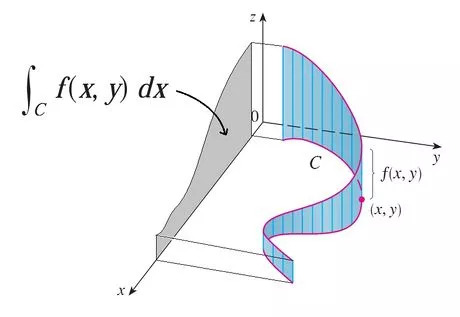
\includegraphics[scale=0.40]{immagini/line.jpg}
		
	\end{center}
	\subsubsection{Lunghezza dell'arco}
	La lunghezza dell'arco di curva r(t) :
	$$\textit{lunghezza arco di curva}=\int_a^b||r'(t)||$$
	\section{Funzioni vettoriali a valori reali}
	Una funzione vettoriale a valori reali è una funzione del tipo $f: \Rn \rightarrow \R$. Il grafico di una funzione vettoriale a valori reali è : $$\text{grafico di }f:\{(x,f(x))\in \R^{n+1}\}$$
	\begin{definizione}
		Ipersuperficie di livello o Curve di livello \\
		$$f: \Rn \rightarrow \R \ \ \ \forall z \in \R \ \ \ c_z=\{x\in \Rn : f(x)=z\}$$ 
	\end{definizione}
	$\fn$ \\
	continuità : vale la definizione generale ( somma , differenza , prodotto di funzioni continue è continua ) 
	
	\begin{teo}{Degli zeri}{}
		
		Sia $\fn$ continua con A insieme aperto e connesso per archi \ref{def:1}. \\
		Supponiamo che per $x,y \in A $ si abbia $f(x) \cdot f(y)<0$ Allora $ \exists z \in A : f(z)=0$
	\end{teo}
	\begin{teo}{Di Weierstrass}{}
		
		$\fn$ continua , con A chiuso e limitato ; Allora f ammette massimo e minimo assoluti in A , ovvero esistono $x_m,x_n \in A$ tali che $$f(x_m) \leq f(x) \leq f(x_n)$$
	\end{teo}
	\begin{teo}{Del valor medio ( Teorema di Lagrange())}
		sia $\fn$ , A aperto e convesso \ref{def:2}. Supponiamo che f sia differenziabile in A , allora per ogni coppia di punti $x,y \in A$ , esiste un punto $c \in A $ tale che : 
		$$f(y)-f(x)=\nabla f(c) \cdot (y-x)$$
		In particolare , $|f(y)-f(x)|\leq ||\nabla f(c)|| \ ||y-x||$ 
		
	\end{teo}
	\subsection{Limiti}
	\begin{definizione}
		Sia $\fn$ definita almeno in un intorno sferico di $X_0\in \Rn$ e sia $ L \in \R^*$. Diremo allora che : $$\lim_{x\rightarrow x_0}f(x)=L$$
		se $\forall \ \{x_k\}_{k=1}^\infty$ di punti di $\Rn:x_k \rightarrow x_0 \ per \ k \rightarrow \infty ( \ con \ x_k \neq x_0 \ \forall k)$ si ha che : $$\lim_{k\rightarrow \infty}f(x_k)=L$$
	\end{definizione}
	\begin{definizione}
		Continuità \\
		Sia $f: \D \subseteq\to \Rn , c\in D$. Diciamo che f è \textbf{continua} in $c$ se e solo se :      
		$$\forall \{x_n\} \subseteq \D: x_n \to c \  \text{abbiamo che }f(x_n)\to f(c)$$
	\end{definizione}
	\begin{teo}{Del confronto}{}
		siano $ f,g,h ; A \subseteq \Rn \rightarrow \R \ \ \ c \in A $ , supponiamo che : \begin{itemize}
			\item $f(x) \leq h(x) \leq g(c) \ per \ x \rightarrow c$
			\item $f(x) \rightarrow l \in \R \ per \ x \rightarrow c $
			\item $g(x) \rightarrow l\in \R \ per \ x \rightarrow c$
		\end{itemize}
		allora $ h(x) \rightarrow l \ per \ x \rightarrow c $
	\end{teo}
	\begin{teo}{Di permanenza del segno}
		Sia $\fn$ definita almeno in un intorno sferico di $x_0 \in \Rn$. Supponiamo che esista : $$\lim_{x\rightarrow x_0}f(x)=L\in \R^*$$
		\begin{enumerate}
			\item se $L>0$ allora $f(x)$ si mantiene positiva almeno in un intorno di $x_0 \in \Rn$ , cioè esiste $\delta > 0 $ tale che $f(x) > 0  \ \text{purchè} \ 0<|x-x_0|<\delta$
			\item Se $f(x) \geq 0$ in un intorno di $x_0$ ( salvo al più $x_0$) allora $ L \geq 0 $ Notiamo che non si puà affermare che $L>0$. anche se $f(x) > 0$
			\item se $f(x)$ è continua in $x_0\ e \ f(x) > 0 $ allora $f(x) $ si mantiene positiva almeno in un intorno $x_0$ , cioè esiste $\delta > 0 $ tale che $f(x) > 0  \ \text{purchè} \ 0<|x-x_0|<\delta$
		\end{enumerate}
	\end{teo}
	Osservazione : \\
	I seguenti insieme sono aperti : 
	\begin{align*}
		A= \{x\in \Rn | f(x) > 0\}\\
		B=\{x\in \Rn | f(x) < 0\}\\
		C=A \cup B =  \{x\in \Rn | f(x) \neq 0\}
	\end{align*}
	I seguenti insiemi sono  chiusi : 
	\begin{align*}
		A=\{x\in \Rn | f(x) \geq 0\}\\
		B= \{x\in \Rn | f(x) \leq 0\}\\
		C=A\cap B=\{x\in \Rn | f(x) = 0\}\\
	\end{align*}
	\subsubsection{Calcolo dei limiti}
	\paragraph{Restrizione di una funzione ad una curva e non esistenza del limite}\hspace{1cm}\\
	Se $\fn$ è un funzione reale di n variabili , $r: I \subseteq \R \rightarrow\Rn$ è una arco di curva in $\Rn$ ed esiste la funziona composta $$g(t)=f(r(t))$$
	questa si dice \textit{restrizione di f alla curva} \textbf{r}
	Per dimostrare che il limite per $x \rightarrow x_0$ di una certa funzione f(x) non esiste è sufficiente determinare due curve che passano da $x_0$ , lungo le quali la funzione tende a due limiti diversi.
	\paragraph{Provare l'esistenza di un limite}\hspace{1cm}\\
	\begin{teo}{}{}
		\label{teorema:1}
		Sia $\fn$ definita almeno in un intorno d i$x_0$ e sia $ L \in \R$ se $g(0,+\infty) \rightarrow \R$ è una funziona tale che $g(\rho)\rightarrow 0 \ per \rho \rightarrow 0 $ e $$|f(x)-L|<g(|x-x_0|)$$   
		per ogni x in un opportuno introno sferico di $ x_0$ allora $$\lim_{x\rightarrow x_0}f(x)=L$$
	\end{teo}
	Per prima cosa calcoliamo il potenziale valore del limiti utilizzando la restrizione di una funzione ad una curva e poi attraverso l'uso di \textit{maggiorazioni con funzioni radiali} ne proviamo l'esistenza. 
	Esempio :\\
	$$\lim_{(x,y)\rightarrow(0,0) }\frac{2x^2y}{x^2+y^2} $$
	ci restringiamo a (x,0) quindi $$\lim_{(x,0) \rightarrow(0,0)}\frac{2x^2 \cdot 0}{x^2+0}=0$$
	Ora per dimostrarlo , riscriviamo la funzione in coordinate polari 
	$$\frac{2x^2y}{x^2+y^2}=\frac{2\rho^3 cos^2(\theta)sin(\theta)}{\rho^2}$$
	utilizzando poi il Teorema \ref{teorema:1} abbiamo che: 
	$$\left | \frac{2x^2y}{x^2+y^2}\right |=\left|\frac{2\rho^3 cos^2(\theta)sin(\theta)}{\rho^2}\right |= 2\rho |cos^2\theta sin\theta| \leq 2 \rho$$
	quindi $2\rho \rightarrow 0 \ \ \rho \rightarrow 0$ allora $$\lim_{(x,y)\rightarrow(0,0) }\frac{2x^2y}{x^2+y^2}=0$$
	\subsection{Differenziabilità}
	\begin{definizione}
		\textit{Derivata direzionale}\\
		Sia $\fn$ , A aperto , $c \in A$ , $v \in \Rn$ un versore. Sia $r(t)=c+vt$ la retta passante per c con direzione v e sia $g(t)=f(r(t))$. Definiamo la derivata direzionale di f nel punto c e nella direzione v.
		$$D_Vf(c)=g'(0)=\lim_{t\rightarrow 0} \frac{f(c+tv)-f(c)}{t}$$
	\end{definizione}
	\begin{definizione}
		\textit{ Derivata Parziale}\\
		Sia $\fn$ , A aperto , $c \in A$ . Diciamo derivata parziale di f : $$\frac{\partial f}{\partial x_i}(c)=D_{e_i}f(c)=\lim_{h\rightarrow 0}\frac{f(c+he_i)-f(c)}{h}$$
		Derivata direzionale nella direzione coordinata $e_i=(0 ,, \dots , 1 , \dots , 0)$. \\
		Altre notazioni equivalenti sono : $\partial_{x_i}f,D_{x_i}f,D_i f , f_{x_i}$
	\end{definizione}
	\begin{definizione}
		Gradiente : 
		è il vettore che collezione le derivata parziali : 
		$$\nabla f(c)=(\partial_{x_1} f , \partial_{x_2}f,\dots,\partial_{x_n}f(c))$$
	\end{definizione}
	\begin{definizione}
		Derivabilità \\
		F è derivabile ( ammette derivate parziali ) se esiste il gradiente di f 
	\end{definizione}
	
	\begin{definizione}
		Differenziabilità \\
		sia $\fn$ , A aperto , $c \in A$. Diciamo che f è differenziabile in c se e esiste un vettore $a \in \Rn $ tale che : 
		\begin{align*}
			&f(c+h)=f(c)+a \cdot h +o(||h||) \ \ \ h \rightarrow 0 \\
			&\lim_{h\rightarrow 0}\frac{f(x_0+h)-f(x_0)-a\cdot h}{||h||}=0\\
			&f(x)=f(x_0)+a \cdot (x-x_0) + o (||x-x_0||) \ \ \ x \rightarrow x_0\\
			&\lim_{x\rightarrow x_0}\frac{f(x)-f(x_0)-a\cdot (x-x_0)}{||x-x_0||}=0\\
		\end{align*}
	\end{definizione}
	\begin{proposizione}
		Se f è differenziabile in $x_0$ , allora f è derivabile in $x_0$ e il vettore \textbf{a} è il gradiente calcolato un $x_0$ :
		$$a=\nabla f(x_0)$$
	\end{proposizione}
	\begin{definizione}
		Se f è differenziabile in $x_0$, si dice differenziale di f calcolato in $x_0$ l'applicazione lineare $df(x_0):\Rn \rightarrow \R$ definita da : $$df(x_0):\mapsto \nabla f(x_0)\cdot h$$
	\end{definizione}
	\begin{definizione}
		Iperpiano tangente \\
		Se f è differenziabile in $x_0$ si dice \textit{iperpiano tangente} al grafico di f in $x_0$ , ilpetrpiano 
		\begin{align*}
			z=f(x_0)+\nabla f(X_0) \cdot (x-x_0)\\
			z=f(x_0)+\sum_{i=1}^n\frac{\partial f}{\partial_{x_i}}(x_0) \ (x-x_i^0)   \end{align*}
	\end{definizione}
	La differenziabilità è una condizione più forte sia della continuità sia della derivabilità.
	Però la differenziabilità non è facile da verificare direttamente. In caso n=2 la differenziabilità $(x_0,y_0)$ significa provare che : $$\lim_{(h,k)\rightarrow (0,0)}\frac{f(x_0+h,y_0+k)-f(x_0,y_0)-\frac{\partial f}{\partial_x}(x_0,y_0)\ h-\frac{\partial f}{\partial_y}(x_0,y_0)\ k}{\sqrt{h^2+k^2}}$$
	\begin{teo}{Della differenziabilità totale , condizione sufficiente di differenziabilità}{}
		Siano $\fn$ , con A aperto e $x_0 \in A$. Supponiamo che le derivate parziali di f esistano in un intorno di $x_0$ e siano continue in $x_0$ . Allora f è differenziabile. \\
	\end{teo}
	\begin{teo}{Formula del gradiente}{}
		Sia $\fn$ , A aperto , $c \in A \ , \ v \in \Rn $. Supponiamo che \textbf{f sia differenziabile} in c. Allora $$D_vf(c)=\nabla f(c) \cdot v=\sum_{i=1}^n \frac{\partial f}{\partial x_i}(c) \cdot v_i$$
	\end{teo}
	\begin{proof}
		f è differenziale in c , $f(c+h)=f(c)+\nabla f(c) \cdot h+o(||h||)$ sia $h=tv$ per $t \in \R$ se $t \rightarrow 0 \ allora \ h \rightarrow 0$ \\
		\begin{align*}
			&f(c+tv)-f(c)=\nabla f(c) \cdot (tv)+o(t) \ \ \ t  \rightarrow 0 \\
			&\frac{f(c+tv)-f(c)}{t}=\nabla f(c) \cdot v+\frac{o(t)}{t} \ \ \ t  \rightarrow 0 \\
			&D_vf(c)=\nabla f(c) \cdot v 
		\end{align*}
	\end{proof}
	\begin{corollario}
		Direzioni di massima e minima crescita \\
		Sia $\fn$ con A aperto di $\Rn$ , f differenziabile in $x_0\in A$. Allora il vettore $\nabla f(x_0)$ indica la direzione e il verso di massimo accrescimento di f , ossia la direzione corrispondente alla massima derivata direzionale : $-\nabla f(x_0)$ indica la direzione corrispondente alla minima derivata direzionale : infine , nella direzione ortogonale al gradiente le derivate direzionali sono nulle- 
	\end{corollario}
	\begin{definizione}
		Massimo e minimo locale \ globale \\
		Sia $\fn$ e $x_0 \in A$ Diciamo che : 
		\begin{enumerate}
			\item $x_0$ è punto di massimo ( minimo) assoluto per f in A e che $f(x_0)$ è il massimo ( minimo) assoluto o globale di f in A se $$\forall x \in A : f(x) \leq f(x_0)\ \  ( f(x_0) \leq f(x))$$
			\item $x_0$ è punto di massimo  (minimo) relativo o locale per f e che $f(x_0)$ è massimo ( minimo) relativo o locale di f se esiste un intorno U di $x_0$ tale che : $$ \forall x \in U : f(x) \leq f(x_0) \ \  (f(x_0) \leq f(x))$$ 
		\end{enumerate}
	\end{definizione}
	\begin{teo} {	Di Fermat }{}
		Sia $\fn$ , con A aperto e $x_0 \in A$ un punto di massimo o minimo locale per f. Se f è derivabile in $x_0$, allora $\nabla f(x_0)=0$ 
	\end{teo}
	I punti in cui si annulla il gradiente sono detti punti stazionari/ critici. Come per il caso in una dimensione non tutti i punti critici sono massimi e minimi. Introduciamo quindi il punto di sella 
	\begin{definizione}
		Punto di sella \\
		Sia $\fn$ , con A aperto e $x_0 \in A$. $x_0$ è un punto di sella se per f esistono due direzioni $v_1,v_2 \in \Rn$ tali che : \begin{align*}
			g_1(t)=f(c+v_1t)\ \ \text{ammette un massimo per } t=0 \\
			g_2(t)=f(c+v_2t) \ \ \text{ammette un minimo per } t=0    \end{align*}
		se non è un punto ne di massimo e minimo 
	\end{definizione}
	\subsubsection{Derivata parziale di secondo ordine}
	Se provvediamo a calcolare la derivata parziale rispetto a una delle
	variabili del gradiente della funzione $f(x,y)$ rispetto una
	delle variabili abbiamo una derivata parziale di secondo ordine. 
	Indichiamo la derivata parziale del secondo ordine con i seguenti simboli :
	\begin{align*}
		\frac{\partial^2f}{\partial x^2}=\frac{\partial}{\partial x}(\frac{\partial f}{\partial x })=f_{xx}  \\
		\frac{\partial^2f}{\partial yx}=\frac{\partial}{\partial y}(\frac{\partial f}{\partial x })=f_{xy}\\
		\frac{\partial^2f}{\partial xy}=\frac{\partial}{\partial x}(\frac{\partial f}{\partial y})=f_{yx}\\
		\frac{\partial^2f}{\partial y^2}=\frac{\partial}{\partial y}(\frac{\partial f}{\partial y })=f_{yy}
	\end{align*} 
	\begin{definizione}
		Matrice hessiana \\
		Data una funzione $\fn$ se tutte le derivate parziali seconde esistono allora si definisce la matrice hessiana della funzione f la matrice $Hf(x)$ data da : 
		$$Hf=\begin{pmatrix}
			\vspace{0.2cm}
			\frac{\partial^2f}{\partial x_1^2} & \frac{\partial^2f}{\partial x_1 \partial x_2} & \dots & \frac{\partial^2f}{\partial x_1 \partial x_n} \\ \vspace{0.2cm}
			\frac{\partial^2f}{\partial x_2 \partial x_1} & \frac{\partial^2f}{\partial x_2^2 } & \dots & \frac{\partial^2f}{\partial x_2 \partial x_n} \\ \vspace{0.2cm}
			\vdots & \vdots & \ddots & \vdots \\
			\frac{\partial^2f}{\partial x_n^2} & \frac{\partial^2f}{\partial x_n \partial x_2} & \dots & \frac{\partial^2f}{\partial x_n^2} \\
			\textbf{}
		\end{pmatrix}\ \ \ \ ,\ \ \ \ (Hf)_{ij}=\frac{\partial^2f}{\partial x_i \partial x_j}$$
	\end{definizione}
	
	
	
	
	\begin{teo}{Di Schwarz }{}
		\label{teo:2}
		Sia $\fn$ , con A aperto.Supponiamo che per certi indici $i,j \in \{1,2,\dots,n\}$ le derivate seconde miste $f_{x_ix_j}.f_{x_jx_i}$ esistano un intorno di un punto $x_0$ e siano entrambe continue in $x_0$ ; allora esse coincidono in $x_0$. \\In particolare se le derivare secondo miste $f_{x_ix_j}.f_{x_jx_i}$ esistono e sono continue in A , allora esse coincidono in tutto A  
	\end{teo}
	Sotto le ipotesi del teorema \ref{teo:2} , l'hessiana di f è una matrice simmetrica in ogni punto di A 
	\begin{definizione}
		Differenziale secondo \\
		Se $f \in C^2(A) \ e \ x_0 \in A$ si dice \textit{differenziale secondo di $f$ in $x_0$} la funzione ; 
		\begin{align*}
			&d^2f(x_0):\Rn \rightarrow \R \\
			&h \mapsto h^tH_f(c)h=\sum_{i=1}^n \sum_{j=1}^n  \frac{\partial^2f}{\partial x_i x_j}(c) \ h_i h_j
		\end{align*}
	\end{definizione}
	\begin{teorema}
		Formula di Taylor con resto di Lagrange \\
		Sia $\fn$ , A aperto e convesso , $f \in C^2(A)$. Sia $c \in A\ , \ h \in \Rn$ tale che $c+h \in A$. Allora $\exists \delta \in (0,1) $ , dipendente da c e h , tale che 
		$$f(c+h)=f(c)+\nabla f(c) \cdot h +\frac{1}{2} h^t H_f (c+\delta h)h$$
	\end{teorema}
	
	\begin{teorema}
		Formula di Taylor con resto di Peano \\
		Sia $f \in C^2(A) \ , \ \forall c \in A$ vale :
		$$f(c+h)=f(c)+\nabla f(c) \cdot h +\frac{1}{2} h^t H_f (c)h+o(||h^2||)\ \ \ \ \ h \rightarrow 0$$
	\end{teorema}
	\begin{teorema}
		Formula di Taylor \\
		Sia $f:\Omega \subset \Rn \rightarrow \R $ di classe $C^k(\Omega)$ dove $\Omega$ è un insieme aperto. Allora in un intorno $a \in \Omega$ : 
		$$f(x)=\sum_{|\alpha|\leq k}\frac{D^{\alpha}f(a)}{\alpha !}(x-a)^\alpha + \sum_{|\alpha|=k}R_{\alpha}(x)(x-a)^\alpha $$ 
	\end{teorema}
	\subsubsection{Studio della natura dei punti critici}
	\begin{teorema}
		Sia $q(h)=h^TMh$ una forma quadratica in $\Rn$. \\Se q è definita postiva allora $$q(h) \geq \la_{min}||h||^2 \ \ \ \ \forall h \in \Rn$$ Se q è una forma definita negativa , allora $$q(h)\leq \la_{max}||h||^2 \ \ \ \ \forall h \in \Rn$$
	\end{teorema}
	\begin{teorema}
		Sia $f \in C^2(A)$ e $x_0 \in A$ un punto critico per f ($\nabla f(x_0)=0$). Se la forma quadratica $$q(h)=h^TH_f(x_0)h$$ è :
		\begin{enumerate}
			\item Definita positiva ( negativa ) allora $x_0$ è un punto di minimo (massimo) locale forte 
			\item Indefinita , allora $x_0$ è un punto di sella 
			\item Semidefinita positiva o negativa , allora il criterio è inconcludente 
		\end{enumerate}
	\end{teorema}
	\begin{teorema}
		dei moltiplicatori di Lagrange \\
		Siano $f,g \in C^1(\R^2)$ e $(x^*,y^*)$ punto di estremo vincolato sotto il vincolo $g(x,y)=b$\\
		Se $(x^*,y^*)$ è regolare per il vincolo cioè $\nabla g(x^*,y^*)\neq 0$ allora esiste $\la^* \in \R$ tale che : 
		$$\nabla f(x^*,y^*)=\la^* \nabla g(x^*,y^*)$$
	\end{teorema}
	Introducendo la funzione $$\mathcal{L}(x,y,\la)=f(x,y)-\la[g(x,y)-b]$$ 
	Il teorema afferma che se $(x^*,y^*)$ è un punto di estremo vincolato , allora  esiste $\la^*$ tale che il punto $(x^*,y^*,\la^*)$ sia un punto critico libero per $\mathcal{L}$ Infatti i punti critici di L sono soluzioni del sistema $$\begin{cases}
		\mathcal{L}_x=f_x-\la_x=0 \\
		\mathcal{L}_y=f_y-\la_y=0 \\
		\mathcal{L}_x=b-g=0 \\
	\end{cases}$$
	Il modo di procedere è il seguente : 
	\begin{enumerate}
		\item Si isolano gli eventuali punti non regolari dell'insieme $g(x,y)=b$ che vanno esaminati a parte
		\item si cercano i punti critici liberi della Lagrangiana e cioè le soluzioni del sistema 
		\item Si determina a natura dei punti critici, A questo proposito risulta spesso utile ( se possibile ) applicare il teorema di weierstrass
	\end{enumerate}
	\subsection{Funzioni Implicite}
	\begin{teo}{Di Dini o della funzione implicita}{}
		Sia $A \subseteq \R^2$ e sia $f: A \rightarrow \R$ un funzione di classe $C^1(A)$.Sia $(x_0,y_0)\in A$. \\Supponiamo che $f(x_0,y_0)=0$ e $\partial_yf(x_0,y_0)\neq 0$.\\
		Allora esiste un intorno I di $x_0$ e un'unica funzione $g : I \rightarrow \R$ tale che 
		$$y_0=g(x_0) \ e \ f(x,g(x))=0 \ \forall x \in I$$
		Inoltre $g\in C^1(I)$ e $$g'(x)=-\frac{f_x(x,g(x))}{f_y(x,g(x))}\ \ \ \forall x \in I$$
	\end{teo}
	\begin{teo}{Di Dini nel caso n-dimensionale  }{}
		$A \subseteq \R^{n+1}$ , A aperto , $f: A \rightarrow R$  un funzione di classe $C^1(A)$.  \\Supponiamo che $f(x_0,y_0)=0$ e $\partial_yf(x_0,y_0)\neq 0 \ \ x_0 \in \Rn \ \ y_o \in \R$.\\
		Allora esiste un intorno U di $x_0 \in \Rn$ e un'unica funzione $\varphi : U\rightarrow \R$ tale che  $$f(x,\varphi(x))=0 \ \forall x \in U$$
		Inoltre $g\in C^1(I)$ 
		$$\frac{\partial\varphi '}{\partial x_j}(x)=-\frac{f_{x_j}(x,\varphi(x))}{f_y(x,\varphi(x))}\ \ \ \forall x \in U \ , \ \forall j=1\rightarrow n$$
	\end{teo}
	\subsection{Integrali}
	\subsubsection{Domini rettangolari}
	\begin{teo}{}{}
		Se $f_[a,b]\times [c,d] \rightarrow \R$ è continua allora è integrabile 
	\end{teo}
	Per una funzione continua e non negativa su un rettangolo , l'integrale doppio ha il significato geometrico di volume della regione tridimensionale compresa fra il piano xy e il grafico della funzione 
	\begin{center}
		\centering
		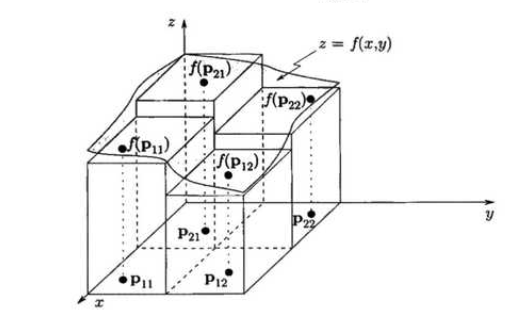
\includegraphics[scale=0.40]{immagini/Screenshot 2024-11-21 at 15.51.25.png}
	\end{center}
	\begin{teo}{Di riduzione , per un rettangolo }{}
		Se $f_[a,b]\times [c,d] \rightarrow \R$ è continua allora il suo integrale doppio si può calcolare come integrale iterato al modo seguente $$\iint_{[a,b]\times [c,d]}f(x,y)dxdy=\int_a^b\left ( \int_c^df(x,y)dy\right)dx =\int_c^d\left ( \int_a^bf(x,y)dx\right)dy $$
	\end{teo}
	\subsubsection{Dominio non rettangolare}
	\begin{definizione}
		Un insieme $E \subset \R$ si dice 
		\begin{itemize}
			\item Insieme \textbf{y-semplice} : 
			$$E=\{(x,y)\in \R : x \in [a,b],g_1(x)\leq y \leq g_2(x)\}$$
			con $g_1,g_2$ funzioni continue 
			\item Insieme\textbf{ x-semplice} ;
			$$E=\{(x,y)\in \R : y \in [c,d],h_1(y)\leq x \leq h_2(y)\}$$
			con $h_1,h_2$ funzioni continue 
			
		\end{itemize}
		E si dice semplice se è y-semplice oppure x-semplice.\\
		E si dice regolare se è unione \textit{finita} di insiemi semplici
	\end{definizione}
	\begin{teo}{}{}
		Sia $\Omega \subseteq \R^2$ un dominio regolare e $f : \Omega \rightarrow \R$ continua. Allora f è integrabile in $\Omega$
	\end{teo}
	\begin{definizione}
		Insieme Misurabile \\
		Un insieme limitato $\Omega \subseteq \R^2$ si dirà \textit{misurabile} se la funzione cotante 1 è integrabile in $\Omega$. In tal caso chiameremo \textit{Misura} di $\Omega$ il numero $$|\Omega|=\iint_{\Omega}1dxdy$$
	\end{definizione}
	\begin{proposizione}
		Sia $g:[a,b]\rightarrow\R $ una funzione continua. Allora il grafico di g è un insieme di misura  nulla
	\end{proposizione}
	\begin{proposizione}
		L'unione di un numero finito di insiemi di misura nulla ha misura nulla
	\end{proposizione}
	\begin{corollario}
		Il bordo di un insieme  regolare ha misura nulla 
	\end{corollario}
	\begin{teo}{}{}
		Sia $\Omega\subseteq \R^2$ un dominio regolare e $f:\Omega \rightarrow \R^2$ una funzione limitata e continua ad eccezione di un insieme di misura nulla di punti di discontinuità.Allora f è integrabile in $\Omega$
	\end{teo}
	\begin{teo}{Di riduzione di funzione discontinue }{}
		Sia $f:[a,b]\times [c,d] \rightarrow \R$ una funzione limita , continua salvo un insieme di misura nulla di punti di discontinuità. Allora il suo integrale doppio si può calcolare come integrale iterato 
	\end{teo}
	\subsubsection{Calcolo degli integrali doppi}
	\begin{teo}{Di riduzione , per domini semplici }{}
		Sia $f : \Omega \rightarrow \R$ continua e sia $\Omega$ un dominio x-semplice , ossia :
		$$\Omega=\{(x,y)\in \R : y \in [c,d],h_1(y)\leq x \leq h_2(y)\}$$
		con $h_1,h_2$ funzioni continue. Allora l'integrale doppio di f si può calcolare come integrale iterata nel modo seguente 
		$$\iint_{\Omega}f(x,y)dxdy=\int_c^d\left(\int_{h_1(y)}^{h_2(y)}f(x,y)dx\right)dy$$
		Se invece $\Omega$ è y-semplice :
		$$\Omega=\{(x,y)\in \R : x \in [a,b],g_1(x)\leq y \leq g_2(x)\}$$ 
		con $g_1,g_2$ funzioni continue  : 
		$$\iint_{\Omega}f(x,y)dxdy=\int_a^b\left(\int_{g_1(x)}^{g_2(x)}f(x,y)dy\right)dx$$
	\end{teo}
	\begin{teo}{}{}
		Sia $d D \subseteq\R^2$ un dominio regolare $f:D\rightarrow \R$ una funzione continua e $T:D'\rightarrow D \ , \ (x,y)=T(u.v) $  con $$\begin{cases}
			x=g(u.v)\\
			y=h(u,v)
		\end{cases}$$
		Una trasformazione di coordinate , o più precisamente , un \textbf{diffeomorfismo globale }.\\
		Allora :$$\iint_Df(x,y)dxdy)\iint_Df(g(u,v),h(u,v))|detJT(u,v)|dudv$$
		Dove JT indica la matrice jacobiana della trasformazione
	\end{teo}
	\subsubsection{Calcolo integrali tripli}
	\paragraph{Integrazione per fili}
	Sia $\Omega$ un dominio di $\R^3$ che si può rappresentare analiticamente in forma 
	$$\Omega=\{(x,y,z)\in \R^3: (x,y)\in D , g_1(x,y)\leq z \leq g_2(x,y)\}$$
	dove D è un dominio regolare nel piano e $g_1,g_2$ sono continue. Allora se $f:\Omega\rightarrow\R$ è una funzione continua , f è integrabile in $\Omega$ e l'integrale si può calcolare mediante la formula
	$$\iiint_\Omega f(x,y,z)dxdydz=\iint_{D}\left(\int_{g_1(x,y)}^{g_2(x,y)}f(x,y,x)dz\right)dxdy$$
	\begin{figure}[h]
		\centering
		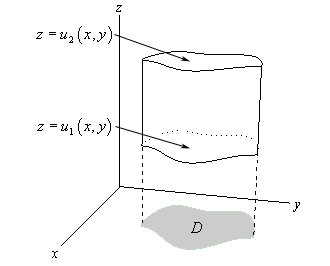
\includegraphics[width=0.5\linewidth]{immagini/Screenshot 2024-11-21 at 16.49.13.png}
		\caption{Integrazione per fili}
		\label{fig:enter-label}
	\end{figure}
	\paragraph{Integrazione per strati}
	Supponiamo ora che $\Omega$ sia un dominio di $\R^3$ rappresentabile nella forma $$\Omega=\{(x,y,z):h_1\leq z \leq h_2 , (x,y)\in \Omega(z)\}$$  $\Omega(z)$ è un dominio regolare nel piano 
	\begin{center}
		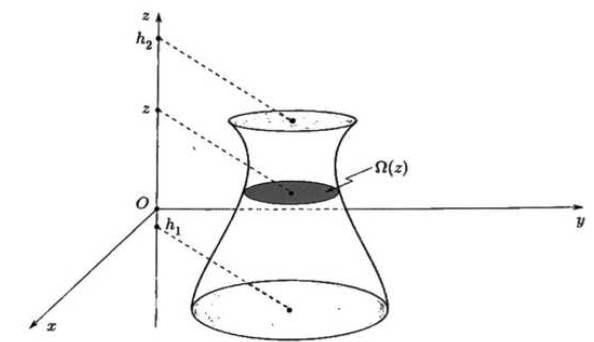
\includegraphics[scale=0.40]{immagini/Screenshot 2024-11-21 at 16.59.38.png}
	\end{center}
	\begin{teo}{Formula di cambiamento di variabili negli integrali tripli }{}
		Sia $d D \subseteq\R^3$ un dominio regolare $f:D\rightarrow \R$ una funzione continua e $T:D'\rightarrow D $un diffeomorfismo globale con  $(x,y,z)=T(u,v,w) $  con $$\begin{cases}
			x=x(u,v,w)\\
			y=y(u,v.w)\\
			z=z(u,v,w)
		\end{cases}$$
		Allora \begin{align*}
			& \iiint_Df(x,y,z)dxdydz= \\
			&=\iiint_{D'}f(x(u,v,w),y(u,v,w),z(u,v,w))|detJT(u,v,w)|du\ dv\ dw
		\end{align*}
		Dove JT indica la matrice jacobiana della trasformazione
	\end{teo}
	\section{Funzione vettoriale a valori vettoriali}
	Funzioni del tipo ; $f: A \subseteq \Rn \rightarrow \R^m$ dove $f(x)=(f_1(x),f_2(x),\dots,f_m(x)) \ \ \ f_i : \Rn \rightarrow R$
	
	\begin{definizione}
		Matrice jacobiana \\
		Sia $\fnm$ , A aperto. La matrice jacobiana della funzione f in $X=(x_1,\dots,x_n)$ è la matrice $\in R^{m\times n}$delle derivate parziali prime della funzione calcolate in x 
		$$Jf(X)=Df(X)=\begin{pmatrix}
			\partial{x_1}f_1 & \dots & \partial_{x_n}f_1\\
			\vdots & \ddots &\vdots \\
			\partial{x_1}f_m &\dots & \partial_{x_n}f_m
		\end{pmatrix} \ (X)$$
	\end{definizione}
	\begin{definizione}
		Una funzione si dice differenziabile in $x_0$ se 
		$$f(x_0+h)-f(x_0)-JF(x_0)h=o(||h||) \ \ \ per \ h\rightarrow 0$$
	\end{definizione}
	\begin{definizione}
		Il differenziale primo di f in $x_0$ è la funzione lineare : 
		\begin{align*}
			df(x_0) \ &: \ \Rn \rightarrow \R^m \\
			df(x_0) \ &: \ h \mapsto Jf(x_0)h
		\end{align*}
	\end{definizione}
	\begin{teo}{Derivata di funzioni composte }{}
		Siano $\fnm$ e $g:B\subseteq \R^m \rightarrow \R^k$ e supponiamo che sia ben definita almeno in un intorno C di $x_0 \in A$ la funzione composta $g \circ f : C \subseteq \Rn \rightarrow \R^k$. \\ Se f è differenziabile in $x_0$ e g è differenziabile in $y_0=f(x_0)$ anche $g \circ f$ è differenziabile in $x_0$ e la sua matrice jacobiana si ottiene come prodotto matriciale delle matrice jacobiane di f e g calcolate nei punti $x_0 \ e \ y_0$ :
		$$J(g \circ f)(x_0)=Jg(f(x_0))Jf(x_0)$$
	\end{teo}
	\begin{teo}{Di Dini , della funzione implicita : caso generale }{}
		Si A un aperto di $\R^{n+m}$, $f:A \rightarrow \R^m$ , $ f \in C^1(A)$ e supponiamo che nel punto $(x_o,y_o) \in A$ sia $$f(x_0,y_0)=0 \ \ \ \ det \ J_yf(x_0,y_0)\neq 0$$
		Allora esistono un intorno $U \subset R^{n+m}\ di \ x_0$ e un'\textbf{unica} funzione $g: U \rightarrow R^m \ , \ g \in C^1(U)$ tale che $\forall x \in U$ 
		\begin{align*}
			&f(x,g(x)) =0 \\
			&Jg(x)= - J_yf(x,g(x))^{-1} \ J_xf(x,g(x))
		\end{align*}
		Data la matrice jacobiana 
		$$Df(x_0,y_0) = \begin{bmatrix}
			\frac{\partial f_1}{\partial x_1}(x_0,y_0) &\dots &\frac{\partial f_1}{\partial x_n }(x_0,y_0) &\vline & \frac{\partial f_1}{\partial y_1}(x_0,y_0) & \dots & \frac{\partial f_1}{\partial y_m}(x_0,y_0) \\ 
			\vdots & \ddots & \vdots & \vline & \vdots & \ddots & \vdots \\ 
			\frac{\partial f_n}{\partial x_1}(x_0,y_0) &\dots &\frac{\partial f_n}{\partial x_n }(x_0,y_0) &\vline & \frac{\partial f_n}{\partial y_1}(x_0,y_0) & \dots & \frac{\partial f_n}{\partial y_m}(x_0,y_0) 
		\end{bmatrix}=\begin{bmatrix}
			D_x & \vline & D_y
		\end{bmatrix}$$
	\end{teo}
	\begin{teo}{	Della funzione inversa  }{}
		Sia $\fnn$ , con A aperto , tale che $f \in C^1(A)$. \\ Supponiamo che per un dato punto di $x_0 \in A$ sia la matrice Jacobiana invertibile : $$det \ \textbf{Df}(x_0)\neq 0$$
		Allora esiste un intorno di $x_0$ e un intorno di V di $f(x_0)$ tra i quali la funzione f è biunivoca; detta $g: V \rightarrow U$ la corrispondenza inversa , si ha che $g \in C^1(V)$ e 
		$$Dg(f(x))=Df(x)^{-1}$$
	\end{teo}
	Nel caso di $ n > 1$ anche se le ipotesi del teorema di invertibilità locale sono soddisfatte da ogni punto del dominio , \textbf{la funzione può non essere invertibile globalmente}. In questo possiamo affermare unicamente che ogni punto ha un intorno in cui la funzione è invertibile , cioè \textbf{la funzione è localmente invertibile}
	\begin{definizione}
		Diffeomorfismo \\
		Sia A un aperto di $\Rn$. Una trasformazione di coordinate $\fnn$ si dice \textbf{diffeomorfismo} ( Diffeomorfismo globale ) se $f \in C^1(A)$ e f è globale invertibile in A e la sua funzione inversa $g:f(A) \rightarrow A$ è $C^1$ nel suo dominio-\\
		Si dice\textbf{ Diffeomorfismo locale } se  $f \in C^1(A)$ e ogni punto $x_0 \in A$ ha un introno $U \subset A$ in cui f è invertibile , con inversa $C^1$
		
	\end{definizione}
	\subsection{Coordinate sferiche}
	$$\begin{cases}
		x=\rho\ sin \varphi \ cos \theta \\
		y=\rho \ sin \varphi\ sin \theta\\
		z=\rho \ cos \varphi 
	\end{cases} \ \ \ \ con \ \rho >0 \ , \ \varphi \in [0,\pi] \ ,\ \theta \in [0,2\pi) $$
	\begin{center}
		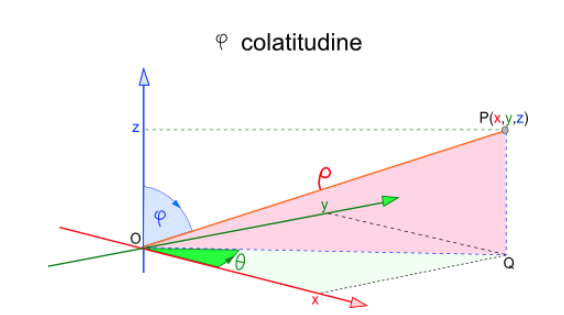
\includegraphics[scale=0.40]{immagini/sferiche1.png}
	\end{center}
	\section{Campi Vettoriali}
	\begin{definizione}
		Campo Vettoriale \\
		Si dice campo vettoriale una funzione $$F:A\subseteq \Rn \rightarrow \Rn$$
	\end{definizione}
	\begin{definizione}
		Dato un campo vettoriale $F:A\subseteq \R^3 \rightarrow \R^3$ con $F\in C^1(A)$ , chiameremo linea di campo  una qualsiasi curva regolare tangente in ogni punto a F
	\end{definizione}
	I punti nei quali escono le linee di campo sono detti sorgenti.\\
	I punti nei quali entrano le linee di campo sono detti pozzi.\\
	Pozzi e sorgenti sono punti singolare per il campo .
	\subsection{Operatori differenziali}
	\begin{definizione}
		Gradiente : Trasforma un campo scalare in un campo vettoriale \\
		$$\nabla=\hat{i}\partial_x +\hat{j}\partial_y+\hat{k}\partial_z$$
	\end{definizione} 

	\begin{definizione}
		Operatore di Laplace  \\
		$$\Delta=\nabla^2=\partial^2_{x_1}+\dots+\partial^2_{x_n} $$
	\end{definizione}
	
	\begin{definizione}
		Rotore : trasforma un campo vettoriale in un altro campo vettoriale \\
		$$\nabla \times F=\begin{vmatrix}
			i & j & k \\
			\partial_x & \partial_y & \partial_z \\
			F_1 & F_2 & F_3 
		\end{vmatrix}= i(\partial_yF_3 -\partial_zF_2)-j(\partial_xF_3 -\partial_zF_1)+k(\partial_xF_2-\partial_yF_1)$$
	\end{definizione}
	\begin{definizione}
		Divergenza : Trasforma un campo vettoriale in un campo scalare\\
		$F:A\subseteq \R^3 \rightarrow \R^3$ con $F\in C^1(A)$ 
		$$divF=\nabla \cdot F=(\partial_x,\partial_y,\partial_z)\cdot(F_1,F_2,F_3)^T=\frac{\partial F_1}{\partial_x}+\frac{\partial F_2}{\partial_y}+\frac{\partial F_3}{\partial_z}$$
		Se la divergenza è uguale a zero allora il campo è detto \textbf{solenoidale} 
	\end{definizione}
	\begin{proposizione}
		$u:\R^3 \rightarrow \R \ , F:\R^3 \rightarrow \R^3 , \ u,F\in C^2(\R^3)$
		\begin{itemize}
			\item $\nabla \times (\nabla u)=0$ il rotore di un gradiente è nullo 
			\item $\nabla \cdot (\nabla \times F)=0$ la divergenza di un rotore è nulla 
			\item $\nabla \cdot (\nabla u)=\Delta u$ La divergenza del gradiente è il laplaciano 
		\end{itemize}
	\end{proposizione}
	\subsection{Lavoro di un campo vettoriale}
	\begin{definizione}
		Lavoro di un campo vettoriale \\
		Sia $\gamma$ un arco di curva regolare , parametrizzata da $r:[a,b]\rightarrow\R^3\ t\mapsto(x(t),y(t),z(t))$ , sia $F:\R^3 \rightarrow \R^3$. Definiamo integrale di linea o lavoro di F lungo $\gamma$ l'integrale :$$\int_{\gamma}F dr=\int_a^bF(r(t))\cdot r'(t) dt=\int_a^b F_1(x(t),y(t),z(t))x'(t)+F_2(x(t),y(t),z(t))y'(t)+F_3(x(t),y(t),z(t))z'(t) dt$$
		Se la curva $\gamma$ è semplice e chiusa , si usa il simbolo $\oint_{\gamma} F dt$\\
		Inoltre a differenza dell'integrale di linea di prima specie , questo integrale dipende dal verso della parametrizzazione della curva $\gamma$
		\subsection{Campi conservativi}
	\end{definizione}
	\begin{definizione}
		Campo conservativo \\
		Un campo vettoriale $F:A\subseteq \R^3\rightarrow\R^3$ si dice conservativo in A se $F\in C^1(A)$ ed esiste una funzione $U:A\rightarrow \R$ , detta potenziale di F , tale che $U \in C^2(A)$ e $F=\nabla U$ in A , cioè $$F_1=\frac{\partial U}{\partial x} \ \ F_2=\frac{\partial U}{\partial y} \ \
		F_3=\frac{\partial U}{\partial z}$$
	\end{definizione}
	\begin{lemma}
		Sia $F=\nabla U$ un campo conservativo in A e sia $\gamma$ una curva regolare a tratti e contenuta in A , parametrizzata da $r:[a,b]\rightarrow A , t\mapsto r(t)$. Siano $p=U(r(a)) \ , \ q=U(r(b))$.
		Il Lavoro di F lungo $\gamma$ è dato da : 
		$$\int_{\gamma}F\cdot dr=p-q $$
	\end{lemma}
	\begin{teo}{di caratterizzazione di campi conservativi}{}
		Sia $F\in C^1(A)$. Le seguenti tre affermazioni equivalenti 
		\begin{enumerate}
			\item per ogni coppia di curve regolari a tratti $\gamma_1 , \gamma_2$ contenute in A e aventi lo stesso punto iniziale e stesso punto finale 
			$$\int_{\gamma_1}F\cdot dr=\int_{\gamma_2}F\cdot dr$$
			\item Per ogni curva chiusa $\gamma$ , semplice , regolare a tratti e contenuta in A $$\oint_{\gamma}F  \cdot dr=0$$
			\item F è conservativo
		\end{enumerate}
	\end{teo}
	
	\begin{teo}{}{}
		Sia $F\in C^1(A)$ e sia A semplicemente connesso. Se $\nabla \times F=0$ ( il campo è irrotazionale) , allora F è conservativo
	\end{teo}
	\subsection{Flusso}
\subsubsection{Superfici}
\begin{definizione}
	Superficie Regolare \\
	Sia $\Sigma$ una superficie parametrizzata da $r : T \subset \R^2 \rightarrow \R^3 , r=r(u,v)$: $\Sigma$ si dice regolare se r è differenziabile ( ogni componente di r è differenziabile) ed inoltre vediamo che la matrice Jacobiana di r ha rango massimo ( in questo caso 2 ). Infine i punti in cui $Dr=\begin{pmatrix}
	x_u & x_v \\
	y_u & y_v \\
	z_u & z_v	\end{pmatrix}=[r_u,r_v]$ non ha rango massimo sono detti punti singolari di  $\Sigma$	\end{definizione}
\begin{definizione}
	Versore normale \\
	Definiamo $n(u,v)=r_u \times r_v \ \forall (u,v) \in T , \hat{n}(u,v)=\frac{n(u,v)}{||n(u,v)||}$ dove $\hat{n}(u,v)$ è detto versore normale a $\Sigma$ nel punto $r(u,v)$.
	\end{definizione}
Quindi $$(x-r_1(u_0,v_0),y-r_2(u_0,v_0),z-r_3(u_0,v_0))\cdot n(u_0,v_0)$$ identifica il pianto tangente a $\Sigma$ passante per il punto $(u_0,v_0)\in T$\\
Esempio : Toro 
$$r(u,v)=\begin{cases}
	(R+rcos(u))\ \cos(v) \\
	(R+rcos(u))\ \sin(v)\\
	r\ \sin(u)
\end{cases} \ \ \ u,v \in [0,2\pi)$$
\begin{definizione}
	Integrale di superficie ( di prima specie) \\
	Sia  $f:\R^3 \rightarrow \R$ e sia $r: T\subset \R^2 \rightarrow \R^3  , r=r(u,v)$ allora possiamo definire 
	$$\iint_{\Sigma}f dS=\iint_T f(r(u,v)) \ ||r_u \times r_v|| du dv$$
	\end{definizione}
\begin{definizione}
	L'area di $\Sigma$ è assegnata dalla formula 
	$$a(\Sigma)=\iint_{\Sigma}1 dS=\iint_T ||r_u \times r_v|| du dv$$
\end{definizione}
\begin{definizione}
	Superficie Orientabile \\
	Una superficie regolare $\Sigma$ si dice orientabile se per ogni curva chiusa e continua $\gamma$ che giace su \s con $\gamma : [a,b] \rightarrow \Sigma$ si ha che $n(\gamma (a)=n(\gamma(b)))$
\end{definizione}
\begin{definizione}
	Flusso \\
	Sia \s una superficie regoalre orientata con versore normale $\hat{n}$.\\Sia $ F : \R^3 \rightarrow \R^3$  un campo vettoriale di classe $C^1$ un introno di \s. \\ Si definisce flusso del vettore F attraverso \s nella direzione e verso $\hat{n}$ l'integrale .
	$$\Phi (F,	\Sigma)=\iint_{\Sigma} F \cdot \hat{n} dS=\iint_T F(r(u,v))\cdot \hat{n}\ ||n(u,v)|| \ d ud v=\iint_T F(r(u,v))\cdot n(u,v) \ d ud v$$
	
	\end{definizione}
\begin{teo}{Teorema di Gauss o della Divergenza}{}
   Sia $D \subset \R^3$ una dominio limitato , semplice rispetto a tutti gli assi , la cui frontiera è una superficie regolare a pezzi e orientabile. Sia $\hat{n_e}$ il versore normale esterno a $\partial D $ e sia D un campo vettoriale di classe $C^1$ su D. Allora vale $$\iiint_{D} \nabla \cdot  F \ dxdydz=\iint_{\partial D} F \cdot \hat{n_e} \ dS$$
\end{teo}
\begin{teo}{Teorema di Stokes o del Rotore }{}
	Sia \s una superficie regolare e orientabile , orientata con il versore normale \textbf{$\hat{n}$} , dotata di bordo $\partial^+ D$ orientato positivamente. \\Supponiamo che $\partial^+ D$ sia una curva regolare , o l'unione di più curve regolari , e sia T il versore tangente a $\partial^+ D$. Sia F un campo vettoriale di classe $C^1$ in un intorno di \s , allora vale $$\iint_{\Sigma} (\nabla \times F)\cdot \hat{n} \ dS=\oint_{\partial^+ D} F \cdot T dl$$ 
	$$\iint_{\Sigma} (\nabla \times F)\cdot \hat{n} \ dS=\oint_{\partial^+ D} F dr$$ 
	Il teorema di Stokes quindi metti in correlazione un'integrale doppio di flusso con un integrale di linea di seconda specie ( quid una circuitazione )
\end{teo}
\begin{teo}{Teorema di Gauss-Green}{}
	Sia D un dominio limitato in $R^2$ che sia semplice rispetto a entrambi gli assi. Sia $F=(P,Q,0)$ un campo vettoriale di classe $C^1(D)$ allora vale la formula : 
	$$\iint_D(Q_x-P_y)dxdy=\oint_{\partial^+ D}P dx + Q dy=\int_a^b P(x(t),y(t))x'(t)+Q(x(t),y(t))y'(t)dt$$
\end{teo}
\section{Serie}
Data una successione $\{a_n \}_n \in \R$ si costruisce la successione delle somme parziali associata ad $\{a_n \}_n \in \R$ come segue :
\begin{align*}
	&s_1=a_1\\
	&s_2=a_1+a_2\\
	&s_3=a_3+a_2+a_1\\
	&\dots\\
	&s_n=a_n+\dots+a_2+a_1
\end{align*}
\begin{definizione}
	Sia $\sum_{n=1}^{\infty}a_n $ una serie e sia $\{s_n \}_n $ la successione delle somme parziali. Allora 
	\begin{enumerate}
		\item se $\lim_{n\rightarrow \infty} s_n=S \in \R$ allora la serie converge e $s=\sum_{n=1}^{\infty} $
		\item se $\lim_{n\rightarrow \infty} s_n=\pm \infty  $ allora la serie diverge
		\item se $\lim_{n\rightarrow \infty} s_n  $ non esiste  allora la serie è irregolare 
	\end{enumerate}
	\end{definizione}
\subsection{Criteri di convergenza per serie a termini positivi}
\begin{teo1*}{Condizione necessaria}{}
	Data una successione $\{a_n \}_n \in \R$ , affinchè la  serie $\sum_{n=0}^{\infty}a_n $ converga è necessario ( ma non sufficiente) che 
	$$\lim_{n\rightarrow \infty }a_n=0$$
\end{teo1*}
Noi ci limiteremo allo studio delle serie a termini non negativi quindi $a_n \geq 0 \ \forall n $\\
Queste serie posso unicamente divergere o convergere poichè la successione delle somme parziali è monotona crescente ( teorema di esistenza del limite nel caso di successioni monotone )
$$s_{n+1}=s_n+a_{n+1} \geq s_n $$
\begin{teo1*}{Criterio del confronto}{}
Date due serie  $\sum_{n=0}^{\infty}a_n $ e $\sum_{n=0}^{\infty}b_n $ con $a_n,b_n \geq 0 \ \forall n$.
\begin{itemize}
	\item se $a_n \geq b_n$ e $\sum_{n=0}^{\infty}b_n=\infty $ allora $\sum_{n=0}^{\infty}a_n= \infty$
	\item se $a_n \leq b_n$ e $\sum_{n=0}^{\infty}b_n < \infty$ allora $\sum_{n=0}^{\infty}a_n < \infty $ 
\end{itemize}
\end{teo1*}
\begin{teo1*}{Criterio del confronto asintotico}
	Se le due successioni $\{a_n\} \ e \ \{b_n\}$  sono asintotiche $a_n ~ b_n$ allora le corrispondenti serie $\sum a_n \ e \ \sum b_n $ hanno lo stesso carattere , cioè o sono entrambe convergenti o sono entrambe divergenti. 
\end{teo1*}
Inoltre possiamo dimostrare per induzione i seguenti risultati:
$$\sum_{n=1}^{\infty}\frac{1}{n^{\alpha}} \ \ \text{converge se } \ \alpha > 1 \ ; \ \text{diverge se } 0 < \alpha \leq 1 $$
$$\sum_{k=0}^{\infty}x^k \ \ \ \text{converge se } |x| < 1  \ \ \ , \ \ \ \text{diverge se } x=1 \ \ \ , \ \ \ \text{indeterminata se } x<-1$$ 
\begin{teo1*}{Criterio della radice }
 Sia $\sum a_n$ una serie a termini non negativi. Se esiste il limite 
 $$\lim_{n\rightarrow +\infty}\sqrt[n]{a_n}=l \ \ \  \begin{cases}
 	l > 1 \ \ \text{La serie diverge } \\ l< 1 \ \ \text{la serie converge} \\ l=1 \ \ \text{il criterio è inconcludente}
 \end{cases}$$
\end{teo1*}
\begin{teo1*}{Criterio del rapporto}
Sia $\sum a_n$ una serie a termini positivi. Se esiste il limite 
$$\lim_{n\rightarrow +\infty} \frac{a_{n+1}}{a_n}=l \ \ \  \begin{cases}
	l > 1 \ \ \text{La serie diverge } \\ l< 1 \ \ \text{la serie converge} \\ l=1 \ \ \text{il criterio è inconcludente}
\end{cases}$$
\end{teo1*}
\subsection{Serie a termini di segno variabile}
\begin{definizione}
	una serie $\sum a_n$ si dirà assolutamente convergente se converge la serie $\sum | a_n|$ 
\end{definizione}
Inoltre vale il seguente teorema
\begin{teo}{}{}
	Se la serie $\sum a_n$ converge assolutamente , allora converge.
\end{teo}
\newpage
\textbf{Serie a termini di segno alternato }
\begin{teo}{Criterio di Leibniz}{}
	Sia data la serie : 
	$$\sum_{n=0}^{\infty} (-1)^na_n \ con \ a_n \geq 0\ \forall n$$
	Sia : 
	\begin{enumerate}
		\item la succesione $\{a_n\}$ è decrescente 
		\item $\lim_{n\rightarrow\infty} a_n=0$
	\end{enumerate}
	Allora la serie è convergente.
\end{teo}

	\begin{definizione}
	Spazio metrico \\
	Diciamo uno spazio metrico la coppia (X,d) dove X è un insieme e $d:X\times X\rightarrow\R$
	\begin{itemize}
		\item $d(x,y)>0 \iff x\neq y$
		\item $d(x,y)=0 \iff x=y$
		\item $d(x,y)=d(y,x)$
		\item $d(x,y) \leq d(x,z)+d(z,y) $ 
	\end{itemize}
\end{definizione}
\begin{definizione}
	Sia (X,d) uno spazio metrico e sia $\{x_n\}_n$ una successione in X.\\
	Diciamo che $\{x_n\}_n$ è di Cauchy se $$\forall \epsilon > 0 \ \ \exists N >0 \ t.c \ \ \ d(x_n,x_m)<\epsilon \ \ \forall n,m >N$$
\end{definizione}
\begin{definizione}
Sia (X,d) uno spazio metrico e sia $\{x_n\}_n\subset X$. \\Diciamo che $x_n\rightarrow x\in X$ se $$\lim_{n\rightarrow +\infty}d(x_n,x)=0$$
\end{definizione}
\begin{definizione}
Spazio metrico completo \\
SIa (X,d) uno spazio metrico. Diciamo che (X,d) è completo se ogni successione di Cauchy è convergente 
\end{definizione}
\begin{definizione}
Diciamo spazio normato la coppia (X,$||\cdot||$) dove X è uno spazio vettoriale ( su campo $\R$) e $||\cdot||:X\rightarrow\R$ è una funzione , detta norma su X , che soddisfa :
\begin{itemize}
\item $||x||>0 \ \ \forall x>0$
\item $||x||=0 \iff x=0$
\item $||\la x||=|\la|\ ||x||$
\item $||x+y||\leq ||x||+||y||\ \ \forall x,y\in X$
\end{itemize}
\end{definizione}
\begin{definizione}
Spazio di Banach \\
Uno spazio di Banach è uno spazio vettoriale normato tale che ogni successione di Cauchy sia convergente a un elemento dello spazio ( cioè lo spazio vettoriale normato è completo rispetto alla metrica indotta)
\end{definizione}
\begin{teo*}{}
	Lo spazio $(C^0(A),||\cdot||_{\infty}) $è uno spazio di banach
\end{teo*}
\subsection{Successioni di Funzioni}
\begin{definizione}
Successione di funzioni 
\end{definizione}
\begin{definizione}
Convergenza puntuale\\
Sia $\{f_n\}$ una successione di funzioni $f_n:A \rightarrow \R$  e sia $f:A\rightarrow \R$.Diciamo che $f_n\rightarrow f$ puntualmente se $$f_n(x)\rightarrow f(x) \ \ \ \forall x \in A$$
\end{definizione}
\begin{definizione}
Convergenza uniforme\\
Sia $\{f_n\}$ una successione di funzioni $f_n:A\rightarrow\R$ e sia $f:A\rightarrow \R$. Diciamo che $f_n\rightarrow f$ su A se 
$$\forall \epsilon > 0 \ \ \exists N>0\ \ t.c \ \ d(f_n(x)-f(x))<\epsilon \ \forall x \in A , \forall n > N$$
\begin{figure}[h]
\centering
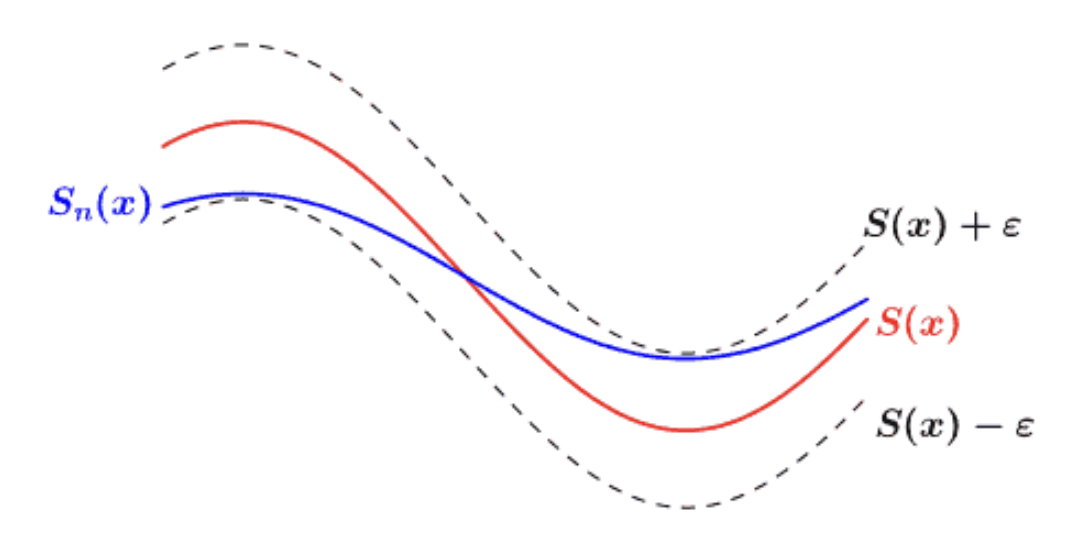
\includegraphics[scale=0.30]{immagini/uniforme}
\caption{Convergenza uniforme }
\end{figure}
\end{definizione}
Se $f_n \in C^0(A)$, allora $f_n \rightarrow f$ uniformemente $\iff f_n\rightarrow \R$ nello norma superiore  \\
$f_n\rightarrow f$ nello spazio normato se $||f_n-f||_{\infty}\rightarrow 0 $ se $sup_{x\in A}(|f_n(x)-f(x))\rightarrow 0$
\begin{teo*}{}
Sia $\{f_n\}:n$ una successione di funzioni , supponiamo che $f_n$ sia limitata su A per ogni n e che $f_n\rightarrow f$ uniformemente. Allora f è limitata 
\end{teo*}
\begin{proof}
	Sia $\epsilon=1$ , date che $f_n\rightarrow f$ uniformemente $\exists N >0 $ tale che $$|f_n(x)-f(x)|<1 \ \ \forall n > N \ \ f(x)-1 \leq f_n(x)\leq f(x)+1$$
	Consideriamo $n>N$. Dal momento che $f_n$ è limitata esiste $M_n\in \R $ tale che $|f_n(x)|<M_n \ \ \forall x \in A$.\\
	Ora $$|f(x)|=|f(x)-f_n(x)+f_n(x)|\leq |f(x)-f_n(x)|+|f_n(x)|\leq 1+M_n \ \ \ \forall x\in A$$
	f è limitata 	
\end{proof}
\begin{teo}{}{}
Sia $\{f_n\}:n$ una successione di funzioni $f_n: A \rightarrow\R$ continue , supponiamo che $f_n\rightarrow f$ uniformemente su A. Allora f è continua 
\end{teo}
\subsection{Serie di funzioni }
Data una successione $\{f_n\}$ costruiamo $\sum_{n}^{\infty}f_n$
\begin{definizione}
Convergenza puntuale \\
$f_n:A\rightarrow \R$ , la serie $\sum_{n}^{\infty}f_n$. Diciamo che la serie converge puntualmente se la serie numerica $\sum_{n}^{\infty}f_n$ converge per ogni $x\in A$ fissato.\\
In alternativa Sia $S_n(x)$ la funzione delle somme parziali , ho convergenza puntuale della se serie se $\{S_n\}$ converge puntualmente 
\end{definizione}
Esempi :
$$\sum_{n=1}^{\infty} x^n=\frac{1}{1-x} \ \ \forall x \in (-1,1)$$
$$\sum_{n=1}^{\infty} \frac{sin(3^n x)}{2^n} \ \ \forall x \ fissato \ \ \sum_n \frac{sin(3^n x)}{2^n} \ e' \ comvergente $$
\begin{definizione}
Convergenza totale delle serie \\
$f_n:A\rightarrow \R$ la serie $\sum_{n}^{\infty}f_n$ , supponiamo che esista una successione $\{a_n\}\subset [0,\infty)$ tale che :
\begin{itemize}
\item $|f_n| \leq a_n \ \ \forall x \in A \ \ \forall n$
\item $\sum_{n}a_n$ converge
\end{itemize}
Allora la serie $\sum_n f_n(x)$ converge totalmente .\\
Inoltre $S_n(x)=\sum_{K=1}^{n}f_n(x)$ converge uniformemente 
\end{definizione}
\begin{teo}{}{}
Sia $\sum_{n}^{\infty}f_n$ una serie totalmente convergente e supponiamo che $f_n$ sia continua allora $$f(x)=\sum_{n}^{\infty}f_n(x)$$ è continua
\end{teo}
\begin{teo}{}{}
Sia $\sum_{n}^{\infty}f_n$ una serie totalmente convergente e  $f_n:[a,b]\rightarrow \R$ continue .\\Allora
$$\int_{a}^{b}\left( \sum f_n(x)\right) dx=\sum_n\left(\int_{a}^{b}f_n(x)dx \right)  $$
\end{teo}
\begin{teo}{}{}
$I\subseteq\R \ , \ f_n:I\rightarrow \R$ derivabili.Supponiamo che 
\begin{itemize}
\item la serie $\sum_{n}f_n$ converge puntualmente 
\item la serie $\sum_{n}f'_n$ converge totalmente 
\end{itemize}
Allora 
$$\left( \sum_{n}f_n\right)'=\sum_{n}f'_n$$ 
\end{teo}
\subsubsection{Serie di potenze}
\begin{definizione}
	Serie di potenze di centro $x_0 \in \R$ una serie di funzioni del tipo continue. 
	$$\sum_{n=0}^{\infty}a_n(x-x_0)^n$$
	dove $\{a_n\}$ è una successione a valori reali. Gli $a_n$ si dicono coefficienti della serie di potenze
\end{definizione}
\begin{definizione}[Raggio di convergenza]
Data una serie di potenze $\sum_{n=0}^{\infty}a_n(x-x_0)^n$ e supponiamo che esista 
$$l=\lim_{n\rightarrow\infty}\sqrt[n]{|a_n|} \ \ \ Poniamo \ \ \ R=\begin{cases}
\frac{1}{l} \ \ &se \ l\neq 0,\infty \\
+\infty \ \ &se \ l=0\\
0 \ \ &se \  l=\infty

\end{cases}$$
Allora \begin{itemize}
\item se $|x-x_0|< R$ la serie converge assolutamente 
\item se $|x-x_0| > R $ la serie non converge 
\end{itemize}
\end{definizione}








\end{document}

	
